% Copyright (c) 2023 Michael Kupperman <kupperma@uw.edu>
%
% Redistribution and use in source and binary forms, with or without modification, are permitted provided that the following conditions are met:
%
% 1. Redistributions of source code must retain the above copyright notice, this list of conditions and the following disclaimer.
%
% 2. Redistributions in binary form must reproduce the above copyright notice, this list of conditions and the following disclaimer in the documentation and/or other materials provided with the distribution.
%
% 3. Neither the name of the copyright holder nor the names of its contributors may be used to endorse or promote products derived from this software without specific prior written permission.
%
% THIS SOFTWARE IS PROVIDED BY THE COPYRIGHT HOLDERS AND CONTRIBUTORS “AS IS” AND ANY EXPRESS OR IMPLIED WARRANTIES, INCLUDING, BUT NOT LIMITED TO, THE IMPLIED WARRANTIES OF MERCHANTABILITY AND FITNESS FOR A PARTICULAR PURPOSE ARE DISCLAIMED. IN NO EVENT SHALL THE COPYRIGHT HOLDER OR CONTRIBUTORS BE LIABLE FOR ANY DIRECT, INDIRECT, INCIDENTAL, SPECIAL, EXEMPLARY, OR CONSEQUENTIAL DAMAGES (INCLUDING, BUT NOT LIMITED TO, PROCUREMENT OF SUBSTITUTE GOODS OR SERVICES; LOSS OF USE, DATA, OR PROFITS; OR BUSINESS INTERRUPTION) HOWEVER CAUSED AND ON ANY THEORY OF LIABILITY, WHETHER IN CONTRACT, STRICT LIABILITY, OR TORT (INCLUDING NEGLIGENCE OR OTHERWISE) ARISING IN ANY WAY OUT OF THE USE OF THIS SOFTWARE, EVEN IF ADVISED OF THE POSSIBILITY OF SUCH DAMAGE.


\documentclass[]{article}
\usepackage{amsmath, amssymb, amsthm, hyperref, graphicx}
\usepackage[margin=1in]{geometry}
\usepackage{caption} \captionsetup[table]{skip=10pt}

\title{Style and Writing Guide for Reports in AMath 352}
\author{Michael Kupperman}
\begin{document}
\maketitle
\begin{abstract}
    This is a basic style guide for preparing reports in applied mathematics, although it can be easily applied verbatim to many other related fields (computational biology, climatology, neuroscience, data science, etc.). The purpose of this document is to collect many standard conventions and expectations into a single place to better enable you to write technical reports in the style of a scientific article. The guidance here is distilled from best practices from academic and technical writing for mathematical audiences.

Please consult your TA when you have questions.

\end{abstract}
\tableofcontents

\section{Content and major sections}

A paper has five major components. These are Title \& Author information, Introduction, Methods, Results, and discussion. While we list them in this order, the best order to write is:

\begin{enumerate}
    \item Methods (as you develop them)
    \item Results (as you obtain them)
    \item Conclusion (as you contextualize results)
    \item Introduction
    \item Title (and abstract, if applicable)
\end{enumerate}
Many papers use sub-section headings to further provide structure. These are not necessary, but can be helpful for writing and for structuring methods sections.
I like to use them when writing to help guide me, even though I later remove them. Some of the lists of objectives below are helpful for providing the structure.

\subsection{First page heading}
The top of the first page of a report should contain
\begin{enumerate}
    \item Report title. This should be germane and descriptive of the contents. A title has two goals:
          \begin{enumerate}
              \item Inform the reader of the contribution you are making or the problem you are solving.
              \item Get the reader to open your article and read more.
          \end{enumerate}
          Good examples include, but are not limited to:
          \begin{enumerate}
              \item ``A Stochastic Differential Equation SIS Epidemic Model''
              \item ``Reconstruction of ``second order'' Models of Traffic Flow''
              \item ``Spectral analysis of Weighted Laplacians Arising in Data Clustering''
          \end{enumerate}
    \item Author names and institutional affiliations. List your university of institution, and your department if affiliated.
    \item Corresponding author contact information. Since most reports will be written by a single author, this will be you. Include your institutional email address.
\end{enumerate}

\subsection{Abstract}
An abstract is not necessary. Please do not include an abstract unless instructed otherwise.

\subsection{``Introduction'' or ``Overview''}
The purpose of the first section is to address the following points at a high level.
\begin{enumerate}
    \item Motivation. Why is this problem interesting? Why should the reader care?
    \item Background. What other information is relevant to solving this problem that you do not plan to develop. For example, if you are building a mathematical model, other noteworthy modeling or analysis attempts at the phenomena of interest that might inform your approach should be discussed. This should be a brief, high-level overview. For example if you are describing a new algorithm, you might write the following sentence.
    \begin{quote}
        Popular iterative solvers often use Krylov subspace methods, but are not easily generalized to almost-symmetric matrices, $A+\epsilon$ where there is a small perturbation breaking an otherwise symmetric matrix.
    \end{quote}

    \item Outline of the rest of the paper and listing of contributions. What is the technical problem you are trying to solve? How do you plan to solve it? How will you validate your (experimental) results?
          What approach are you going to take?
\end{enumerate}

Not all of these will apply and due to page limits you may not be able to reasonably address all of them. Fortunately, writing introductions is somewhat formulaic if you are familiar and conversational about the literature. For a three-to-five page report, the following three-paragraph structure works well.

\begin{enumerate}
    \item Paragraph 1. Funnel the reader in from a high-level view of the subject, to the specific problem you are addressing. Start to motivate the problem and narrow down to your problem of interest.
    \item Paragraph 2. Introduce the specific research question you are going to solve. Discuss the problem in context of the broader literature. Both domain science and mathematical literature are relevant here. Draw any relevant comparisons to other work.
    \item Paragraph 3. Summarize your plan for the paper. This paragraph usually starts with ``In this paper, we will...'', or ``To answer this question, we ...''.\footnote{When you're reading papers, go look for this type of sentence in the last paragraph of the introduction. It's strikingly common.}
          Sketch, at a high-level, what your methodological approach will be and what your interpretation of these results will be. This is a good place to sketch out your report.
\end{enumerate}
These can be collapsed together into one or two paragraphs depending on style and length constraints. The important thing is to address the three points above.

\subsection{``Methods'' or ``Theoretical background and description of algorithms''}

The later section heading ``Theoretical background and description of algorithms'' is more descriptive and gives us a better springboard to understand this section. The purpose of this section is to document how you performed your analysis and ensure that your work can be \emph{independently} reproduced without examining your code. Write this section around the same time you perform your analysis, so you can document your process. The methods section should address the following points:
\begin{enumerate}
    \item Theoretical background. Now you can get into some detail about the literature or existing knowledge that informs your approach. Introduce any core mathematical concepts that are needed. For this course, if you deploy a new (to you) method, it would be appropriate to briefly introduce the method here. Introduce (briefly) any frameworks you are using (linear algebra, Fourier analysis, dynamical systems, etc.).
    \item Quickly transition to how the method/framework you introduced applies to the problem, explaining how you're using the items introduced in the theoretical background to solve this problem.
    \item Introduce any further algorithms you need to use. \emph{You do not need to give the textbook description of the algorithm}, but you should give a high-level overview of how the algorithm works and how it applies to your problem. If this application isn't obvious to you, take an extra sentence to explain how it will solve the problem.
\end{enumerate}

\emph{The methods section should not contain any results or any code}. If randomization was used in your work (typically to generate data), you do not need to record the random seed in your report. The setting of a random seed in your code is sufficient.

\subsection{``Results'' or ``Computational results''}
Most people read the results section first, when deciding if they want to read the rest of the paper. This is the core of your paper.
While this section usually isn't entirely self-contained, a subject-matter-expert should be able to parse this section without reading the methods section. The purpose of this section is to present your results and discuss them. Introduce each experiment very briefly (if the reader is interested, the details can be found in the methods section). Present the results of the experiment, and discuss them. A good way to develop the discussion section is to start by explaining your results to a fellow student or STEM interested friend. Use that outline to develop your results section.

A well written results section does the following:
\begin{enumerate}
    \item Present the results in a logical order. Start with the logical beginning, and progress. This often does not correspond to the chronological order of your experiments.
    \item Figures and tables should be used \emph{as needed} to communicate results. The main text and your arguments should be understandable without requiring the user to read the figures. Figures should be used to support your arguments, not make them.
    \item Remember that evidence does not explain itself. \emph{You} need to explain what the evidence means, and \emph{how it supports the arguments that you make} to answer the research question.
\end{enumerate}

\subsection{Discussion}

The discussion section has a few aims:
\begin{enumerate}
    \item Provide a higher level summary (key take-away points for the reader) of what you did/what you learned.
    \item Place your result in the context of the broader literature or problem domain. How does your result fit in with the broader literature? What does it tell us about the domain application we are interested in? Are the results indicative of a new paradigm? Do they suggest a fundamentally new approach or issue? Reference back to aspects you will introduce in the introduction.
    \item Address any possible limitations of the approach. Where might you expect the approach to fail to generalize? Did you encounter known or foreseeable issues?
          What assumptions are critical, and how realistic are they in practice? Does your method have limitations on data (e.g. does it require a lot of data, does the computational cost become prohibitive fast necessitating small data)?
    \item Discuss any future work that might be done, but might be out of scope for the project that generated this paper. Usual aspects to consider are larger or smaller data, more complex data, weaker or stronger assumptions, or different applications.
\end{enumerate}

\emph{Be direct about these aspects. It will help your reader understand the value of your contribution.}
A good discussion section for a three to five-page report is two to four paragraphs, addressing the points above in order. A one to three-page report can have one to three paragraphs depending on length constraints and writing style.

\section{Formatting, style, and readability}

Now that we have addressed the information content of the report, we will now address the more mechanical aspects of writing style. These will greatly improve the flow, readability, and overall quality of your report.

\subsection{Main text}
The main text of a scientific report is written in paragraph format, with complete sentences. It is helpful to read your report out loud to test this. If it is difficult to read or for a listener to follow, you should consider revising your writing. Both ``I'' or ``We'' are acceptable to use, however do not mix the two choices. Many authors prefer ``We'' even when writing a single author paper. This is a stylistic choice, and either is acceptable.


Assume the reader has not seen any handouts or the assignment text, but is broadly interested in the problem you are addressing. You do not need to define elementary objects like a matrix, sequence, or a vector.
This may require you to rewrite or typeset equations, or to restate portions of the problem.

\subsubsection{How to use Figures from the main text}
The main text must be readable without needing to view the figures. You should describe any features in the main text that are necessary to understand the results. Figures should be used to support your arguments, not make them. For example, a results section might contain the following text.
\begin{quote}
    The results of this experiment are shown in Figure 2. We see that the algorithm converges in 10 iterations when no noise is present and the error is less than $10^{-6}$. However, when Gaussian noise is added to the same data with a modest $\sigma=0.01$, the algorithm fails to converge after 100 iterations. This demonstrates that our algorithm is dependent on low noise data.
\end{quote}

While the contents of the referenced figure may be very helpful in making the point that the algorithm being investigated is sensitive to noise, the point is made needing the figure. A figure is used to support an argument, not make it.

\subsubsection{Equations}
Equations are often necessary to concisely describe the problem you are solving. Equations should be numbered sequentially and imporant equations should be elevated to equation blocks, then referenced in the main text. For example, the following text
\begin{quote}
    We are interested in solving the following optimization problem
    \begin{equation} \label{eq:opt_ex}
        \min_{x\in\mathbb{R}^n} f(x) \text{ subject to } g(x) = 0
    \end{equation}
    where $f:\mathbb{R}^n\to\mathbb{R}$ is a convex function and $g:\mathbb{R}^n\to\mathbb{R}^m$ is a vector valued function. To solve \eqref{eq:opt_ex}, we will use the method of Lagrange multipliers.
\end{quote}
allows the reader to rapidly identify equation (1) as the problem of interest. It is much more difficult to rapidly identify the problem of interest in the following text.
\begin{quote}
    We are interested in solving the following optimization problem
        $\min_{x\in\mathbb{R}^n} f(x) \text{ subject to } g(x) = 0$
    where $f:\mathbb{R}^n\to\mathbb{R}$ is a convex function and $g:\mathbb{R}^n\to\mathbb{R}^m$ is a vector valued function. To solve this optimization problem for our problem given in the previous paragraph, we will use the method of Lagrange multipliers.
\end{quote}
Equations should be typeset using the equation environment in your document preparation system. Inline equations should only be used for very short expressions, such as $f(x) = x^2$ or $g(x) = 0$.

\subsubsection{Grammar and language checking tools}

It is to your advantage to employ grammar and language checking tools. While broad AI tools are not sufficiently advanced\footnote{Yet. I'm sure they'll be here soon.} to automatically improve your writing, there are many tools that can help you identify grammatical errors and improve the quality of your writing.

While many options exist, the most common are:
\begin{enumerate}
    \item \href{https://www.grammarly.com/}{Grammerly}
    \item \href{https://languagetool.org/}{LanguageTool}
    \item Microsoft Word's built in grammar checker
    \item Ask a friend to read your paper.
\end{enumerate}
If you prefer to write in an IDE (such as VS Code), there are often plugins offering similar functionality.


\pagebreak

\subsection{Figures and Tables}

Figures and tables have similar formatting requirements. Both figures and tables should be numbered sequentially and must be referenced and discussed in the main text.
Let us use the following figure and table as examples. In this example, we would like to present the results of a computational experiment examining how adding a correction term to an algorithm impacts performance.

% Putting our requirements together, we arrive at the following figure.
\begin{figure}[htb!]
    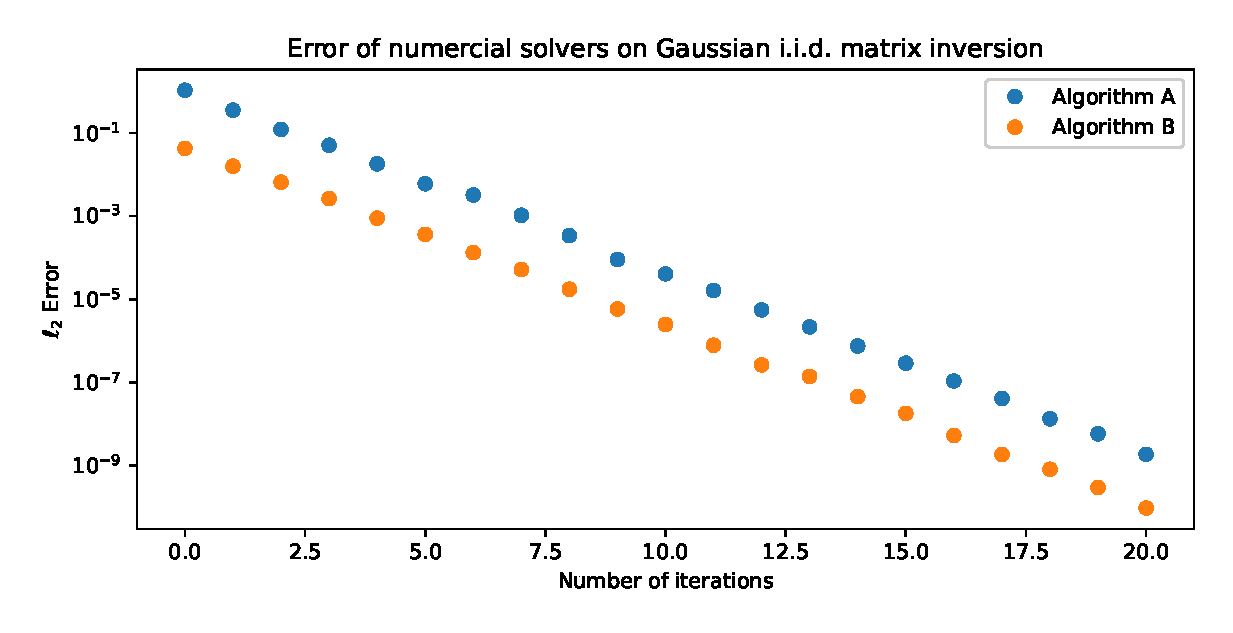
\includegraphics[width=\textwidth]{figure.eps}
    \caption{{\bf The additional corrections in algorithm B do not contribute to a faster rate of convergence.} Computed error of algorithm A and algorithm B as a function of the number of iterations. While algorithm B has a lower error at each iteration, the error of both algorithms decay at the same rate.}
\end{figure}

Suppose we would also like to report the exponential rate of convergence, $e^{-\alpha t}$ of the two algorithms. We can use a table to present this information.


\begin{table}[hb!]
    \centering
    \caption{{\bf Exponential rate of convergence of the two algorithms is unchanged by the additional corrections.} Exponential rate of convergence is defined as $\alpha$ where the error is proportional to $e^{-\alpha t}$, where $t$ is the number of iterations. The data used is visualized in Figure 1.}

    \begin{tabular}{c|c}
        Algorithm & $\alpha$ \\
        \hline
        A & $1.004653$ \\
        B & $0.997469$ \\
    \end{tabular} \\

    *The difference is not statistically significant.
\end{table}


A figure or table has two parts:
\begin{enumerate}
    \item The image or table itself.
    \item A supporting caption.
\end{enumerate}
In a figure, the caption is placed \emph{below} the graphic, while for a table the caption is placed \emph{above} the cell grid. A table note is placed below the table to define terms of offer short additional clarifying remarks.


\subsubsection{Should I use a figure or a table?}
This is a common question when first learning to write articles. There is a simple test for deciding this. \emph{Which matters more, the numerical values or the trends in the data}? If the numerical values matter more, use a table. Common examples of this include presenting summary statistics about a survey population, listing tested material properties for a new material, or comparing a set of performance statistics of a new machine learning algorithm against a previous state-of-the-art algorithm on a benchmark data set. If the trends in the data matter more, use a visualization and place it in a figure. In most science and engineering, a figure is the default option.

\subsubsection{Placement and relation to the main text}
Figures and tables should be referenced in the main text, and should be numbered sequentially. Figures should be placed as close to the text that references them as possible. Figures should be placed at the top or bottom of a page, not in the middle of a paragraph.

\subsubsection{Figure graphics}
For computer generated figure graphics such as plots and charts, figures should generally be saved as a vector graphic. Common formats include PDF, SVG, and EPS. These formats are scalable and will not become pixelated when zoomed in. If your word processor is unable to import vector graphics, a high DPI PNG is acceptable. \emph{Never take a picture of your screen with a phone to make a figure}.

If your figure contains many plots or panels, you may find it convenient to letter each panel. In other cases, it is easier to refer to Figure \# Left and Figure \# Right. This is a stylistic choice, and either is acceptable.
In Python, the standard library for plotting is Matplotlib, but alternatives or extensions can be used, such as Seaborn, Plotly, or Pygal.
Once you have generated a plot in Python, \emph{save the plot to a pdf, svg, and/or eps file}. Then insert the saved file into your document. \emph{Do not take a screen capture of your plot}.

\subsubsection{Plots}
Plots are the primary type of graphic for depicting results in a figure. Plots must be generated using a plotting library. All plots should have the following features.
\begin{enumerate}
    \item Axes labels. Axes labels should be descriptive and informative. For example, if you are plotting the error of an algorithm as a function of the number of iterations, the x-axis might be labeled ``Number of iterations'' and the y-axis should be labeled with the type of error, perhaps ``$\ell_2$ error''.
    \item A legend. If multiple data series are present, a legend should be present that gives the reader information about what each line represents. For example if we are testing the performance of two algorithms, the legend should indicate which line is which algorithm. This can sometimes be placed in the caption, but it is often helpful when coding to place it in an empty regions of the plot.
    \item Title. If there is only one series, the title may be sufficient to indicate what the plot is showing. If there are multiple series, the title should be descriptive of the plot, but not necessarily the data. For example, if we are testing the performance of two algorithms, a good title might be ``Error as a function of iterations''.
\end{enumerate}

\subsubsection{Figure and table captions}

All figures and tables must have a caption. A caption is a short description of the contents of the figure or table. A good caption contains at least two sentences. The first sentence is called the figure/table title, and it summarizes the contents and a take-away message for the figure. Figure titles should be approximately 15  words or less.
A good example of a figure title is the following.
\begin{quote}
    The additional corrections in algorithm B do not contribute to a faster rate of convergence.
\end{quote}

The second sentence provides more detail about the figure or table. This is sometimes called the legend, and it should be descriptive enough that a reader can understand the figure or table at a mechanical level without reading the main text. They should be able to describe what is happening, even if they do not understand the context or significance of the figure or table. A good example of a legend is the following.
\begin{quote}
    Computed error of algorithm A and algorithm B as a function of the number of iterations. While algorithm B has a lower error at each iteration, the error of both algorithms decay at the same rate.
\end{quote}


\end{document}
